\chapter{Data Preparation}

\begin{figure}[hbtp]
	\centering
	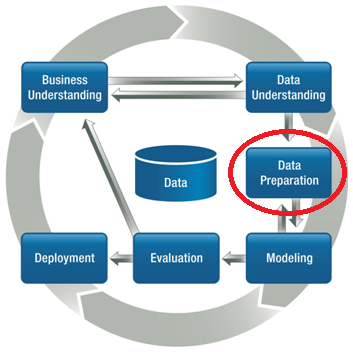
\includegraphics[width=0.4\textwidth]{./images/CRISPDM_3.png}
	\caption{CRISP-DM - Data Preparation}
	\label{CRISPDM_3}
\end{figure}
In questa fase si andranno a modellare i dati presenti nel dataset al fine di poter essere utilizzabili nelle successive fasi del CRISP-DRM.
\section{Criteri di Inclusione/Esclusione dei dati}
La totalità dei dati presenti nel dataset verrà utilizzata per il processo di KDD; non verrà fatta nessuna esclusione di istanza.
\section{Sampling data}
Visto il quantitativo di istanze disponibili (8000 istanze), si è preferito non ridurre la cardinalità delle istanze attraverso il campionamento.
\section{Feature Selection}
\label{Feature Selection}
Per quanto riguarda la fase di feature selection, si è deciso di effettuare una selezione tra gli attributi presenti in quanto, molti di questi, presentano valori nulli nella maggior parte delle istanze del dataset. Questo potrebbe, non solo non portare benefici al processo, ma anche peggiorare l'efficienza dell'algoritmo.

Come algoritmo di feature selection, si è scelto il \textit{CfsSubsetEval}, il quale valuta il miglior subset degli attributi considerando la singola correlazione di ognuno con l'attributo di classe. Si sceglierà il subset con la più alta correlazione con l'attributo di classe, ma allo stesso tempo, con una bassa correlazione con gli altri attributi. La ricerca nello spazio del subset degli attributi viene realizzata attraverso la strategia best first cercando di avvicinarsi ad un risultato ottimale in maniera greedy tagliando lo spazio di ricerca con la tecnica del backtracking.\cite{Hall1998}
L'algoritmo può operare in tre modi:
\begin{itemize}
	\item partire da un insieme di feature vuoto e incrementarlo aggiungendo le più predittive;
	\item partire dall'insieme contenente tutte le feature e ridurlo eliminando quelle meno predittive;
	\item partire da un qualsiasi punto e muoversi in entrambe le direzioni aggiungendo e rimuovendo feature.
\end{itemize}
\section{Construct Data}
Al fine aumentare il quantitativo informativo del dataset, sono state generate nuove istanze attraverso l'utilizzo dell'algoritmo \textit{SMOTE}.
\subsection{SMOTE}
\label{SMOTE}
SMOTE permette di ricampionare il dataset in maniera supervisionata utilizzando la \textbf{S}ynthetic \textbf{M}inority \textbf{O}versampling \textbf{TE}chnique. 
\cite{Chawla02smote:synthetic}. Questa tecnica combina l'\emph{Information Oversampling} della classe minorante, con la \emph{Random Undersampling} della maggiorante. Di seguito l'algoritmo per effettuare il sovracampionamento della classe minorante.
\begin{algorithm}
	\caption{\emph{SMOTE’s Informed Oversampling Procedure}}
	\begin{algorithmic} 
		\FORALL{Minority Sample}
		\STATE Find its k-nearest minority neighbours
		\STATE Randomly select $j$ of these neighbours
		\STATE Randomly generate synthetic samples along the lines joining the minority sample and its j selected neighbours
		(j depends on the amount of oversampling desired) 
		\ENDFOR
	\end{algorithmic}
\end{algorithm}
Il dataset era inizialmente poco bilanciato, in quanto contava su un totale di 8000 istanze, il 39\% di esempi classificati come positivi mentre il restante 61\% come negativi. Con questo algoritmo, invece, il dataset passa da 8000 a 11112 istanze, incrementando il numero di esempi positivi portandolo al 56\% e riducendo al 44\% le istanze negative.
\subsection{Problemi di SMOTE}
\paragraph{Sovra generalizzazione}
SMOTE diventa dannoso nel momento in cui si generalizza alla cieca l'area di minoranza senza tener conto della classe di maggioranza. Questa strategia è particolarmente problematica in caso di alta asimmetricità della distribuzione della classe, poiché in tal caso, la classe di minoranza risulta essere più sparsa rispetto a quella di maggioranza, determinando una maggiore possibilità di classi miste.
%SMOTE’s procedure is inherently dangerous since it blindly generalizes the minority area without regard to the majority class.
%This strategy is particularly problematic in the case of highly skewed class distributions since, in such cases, the minority class is very sparse with respect to the majority class, thus resulting in a greater chance of class mixture.

\paragraph{Mancanza di flessibilità}
Il numero di campioni sintetici generati da SMOTE viene fissato in anticipo, non consentendo alcuna flessibilità del tasso di ri-equilibrio.
%The number of synthetic samples generated by SMOTE is fixed in advance, thus not allowing for any flexibility in the re-balancing rate.

\section{Integrate Data}
La fase di integrazione dati è utile quando si stanno analizzando dati che possono essere descritti meglio con informazioni provenienti da altri database. In questa fase si integrano quindi i dati provenienti da diverse sorgenti al fine di ottenere una base di dati più popolata e quindi più dettagliata. L'integrazione è utile anche quando le informazioni a disposizione sono poche e hanno quindi la necessità di essere espanse con dati esogeni.
In questo caso, non è stato necessario creare attributi derivati.

\section{Format Data}
Il dataset a disposizione era in formato testuale creato usando lo standard CSV il cui parametro di delimitazione delle istanze era il carattere spazio. Questo ha reso necessario una conversione del dataset nel formato standard \emph{ARFF} in modo tale da poter essere utilizzato in Weka.
